\newsection 
\subsection{Modeling}
\label{sec:modeling}

\sectionauthors{Drew A. Hudson, Antoine Bosselut, Alex Tamkin, Omar Khattab, Jared Quincy Davis, Jiaxuan You, Trevor Gale}


\begin{figure}[!ht]     
\centering
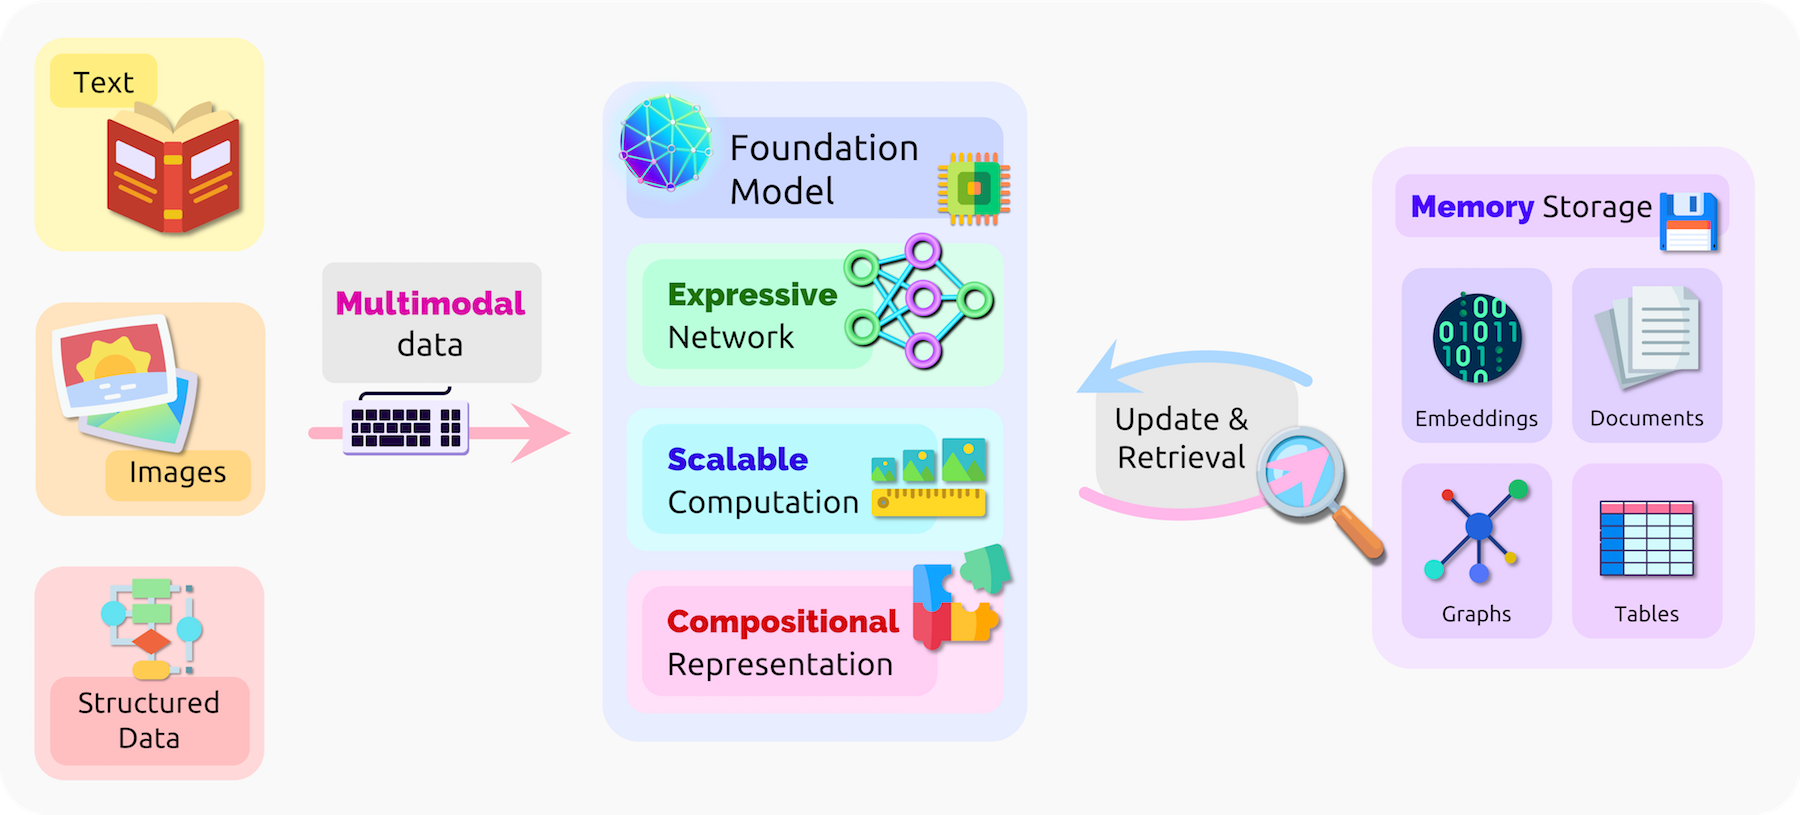
\includegraphics[width=\linewidth]{technology/figures/Modeling_1.png}
\caption{The five key properties of a foundation model:  \textit{expressivity}\dash{}to flexibly capture and represent rich information; \textit{scalability}\dash{}to efficiently consume large quantities of data; \textit{multimodality}\dash{}to connect together various modalities and domains; \textit{memory capacity}\dash{}to store the vast amount of accumulated knowledge; and \textit{compositionality}\dash{}to generalize to new contexts, tasks and environments.}     
\label{fig:modeling} 
\end{figure}

The emerging paradigm of foundation models has attained impressive achievements in AI over the last few years, as models such as BERT \citep{devlin2019bert} shine at a wide spectrum of language understanding tasks: from textual classification and entailment to question answering and reading comprehension, while GPT-3 composes rich and fluent tales about unicorns \citep{brown2020gpt3} and DALL-E  shows signs of visual creativity, generating from scratch strikingly-realistic pictures of avocado chairs \citep{ramesh2021zeroshot}.

These and other instances of recent foundation models not only achieve remarkable performance across a multitude of diverse downstream tasks and applications \citep{squad2,wang2019superglue}, but also manifest noteworthy behaviors of interpretability \citep{stylegan2}, robustness \citep{devlin2019bert}, controllability \citep{styleclip} and generalization \citep{brown2020gpt3}. What does it take for a model to demonstrate such qualities? What architectures are capable of consuming large quantities of potentially multimodal information and translate them into rich knowledge of the world? And overall, what desirable properties should a network possess to give rise to a foundation model?

Here, we identify and discuss five such properties, spanning \textit{expressivity}, \textit{scalability}, \textit{multimodality}, \textit{memory capacity}, and \textit{compositionality}, that we believe are essential for a foundation model in order to: (1)~distill and accumulate knowledge from various sources and domains, (2)~organize it in an effective and scalable representation, and (3)~flexibly generalize it towards novel contexts.  For each of these properties, we motivate their necessity, provide examples of contemporary  models that incorporate them, and explore key challenges and promising avenues  for future research and development. See \reffig{modeling} for an overview diagram.

\subsubsection{Expressivity} 
\label{sec:modeling-expressivity} 

\textit{Expressivity} concerns with the theoretical and practical capacity of a network to model the data distribution it is trained over and represent it in a flexible manner. Prior works have proposed formal expressivity measures to characterize the complexity of functions a network can compute, or more precisely, approximate, which is essentially affected by its depth, width, connectivity, and structural patterns \citep{expressive}.

As the \textit{No Free Lunch} theorem suggests, there is no single model or algorithm that suits best for all cases \citep{lunch}, and so, for our purposes, we are particularly interested in identifying which models could effectively capture the facets of \textit{natural information}, such as human language or real-world images \citep{bengiobook}. These modalities are either continuous (as in vision) or discrete (as in language),  are distinctly hierarchical and high-dimensional, and present a complex set of relations and interactions among their constituent elements, whether these are  pixels, words or physical objects. 

Indeed, recent breakthroughs in generative modeling provide strong evidence for the high expressivity of neural networks, as they successfully express distributions of textual \citep{brown2020gpt3,devlin2019bert,jurassic1,gpt-j}, auditory \citep{Oord2016WaveNetAG}, and visual \citep{stylegan2,biggan} domains, and generate samples of high fidelity, diversity and realism.

\paragraph{Inductive Biases.} Much of the success of neural networks over the last decade in modeling natural data is owed to the \textit{networks' high depths}, as could be roughly measured by the number of stacked non-linear layers they are composed of, or the number of computational steps they take during their chain-of-reasoning.  Great depths play a crucial role in enhancing networks' expressivity, allowing them to form powerful \textit{hierarchical} and \textit{distributed} representations that could generalize from the training data to new unseen examples \citep{he2016resnet,levine2020limits}. 

The \textit{universal approximation theorem} \citep{approx} indeed states that even simple multilayer perceptrons (MLPs) can represent a broad set of functions, while different \textit{inductive biases}, as those implemented in {Recurrent Neural Networks} (RNNs) or {Convolutional Neural Networks} (CNNs) \citep{bengiobook}, can improve the learning efficiency and enhance the capacity of a given network to model different forms of information: sequential data, common to language, speech and time-series, for the former, or spatially-invariant information, as in images or videos, for the latter.

\paragraph{Transformer Networks \& Attention.} Meanwhile, transformer networks \citep{vaswani2017attention}, introduced more recently, demonstrate the importance of capturing \textit{long-range dependencies} and pairwise or higher-order interactions between elements. They build on the \textit{self-attention} mechanism \citep{vaswani2017attention,attention} that enables shorter computation paths and provides direct means to compare elements far-across the input data (such as a pronoun and its antecedent in a sentence, or two sentences that refer to the same topic).

From another perspective, the \textit{multiplicative interaction} embodied in both attention as well as gating structures (as in LSTMs \citep{lstms} or Mixture-of-Experts \citep{moe}) offers a more flexible alternative to the rigid fixed-weight computation of MLPs and CNNs, \textit{dynamically adapting the computation} to the input at hand. This proves especially useful for language modeling, where, for instance, given a sentence like ``She ate the ice-cream with the X", while a feed-forward network would always process it in the very same manner, an attention-based model could adapt its computation to the input\dash{}updating the contextual representation of the word ``ate'' if the prepositional phrase (PP) attachment X is ``spoon'', or instead link it to the ``ice-cream" if X refers \eg to ``strawberries" \citep{ppa}.

\paragraph{General-Purpose Computation.} 
A final notable advantage of attention over prior architectures stems from its stronger \textit{generality}, where it is not strongly tied to a particular task or domain, as is the case for the local receptive field of convolution or the sequential assumption of recurrent networks, both reflecting inherent properties specific to the vision and language modalities respectively. We hypothesize that the general-purpose nature of attention and transformers contributes to their broad applicability for a wide range of research problems and applications \citep{liu2019roberta,visual_transformer,ganformer}.

This contrast captures a more general \textit{trade-off between task-specialization and expressivity}: models with stronger structural priors can leverage them to improve sample efficiency on the particular tasks that benefit from these assumptions; while conversely, models that integrate weaker inductive biases learn more slowly, but can in turn scale to higher volumes of data and adapt to a diverse set of domains, since they do not rely on restrictive or task-specific suppositions. As both data and compute turn more accessible, we observe that the exploration of models with a \textit{minimal set of inductive biases} that can ``let the data speak for itself" seems to serve as a more promising approach for future research in the field.

\paragraph{Challenges \& Future Directions.} Notwithstanding the stellar progress and accomplishments of neural networks in general, and foundation models in particular, in terms of expressivity, notable challenges still remain. Leading approaches \citep{performer,visual_transformer} keep struggling with modeling of extremely long-range dependencies, such as those occurring in books, movies, or even DNA sequences, which may be attributed to the quadratic computation of contemporary transformer-based approaches \citep{wang2020linformer,lin-et-al-2021-naacl}. 

This challenge essentially reflects the \textit{trade-off between efficiency and expressivity}: where explicit modeling of long-distance interactions through short and direct computation paths improves expressivity on the one hand, but comes at the expense of scalability due to computation entailed by the increased connectivity on the other \citep{child2019generating,kitaev2020reformer,performer}. Models such as the GANformer \citep{ganformer} and the Perceiver \citep{jaegle2021perceiver,jaegle2021perceiverio} explore ways to balance these two properties and propose transformers with linear complexity that rely on \textit{bipartite} or \textit{bottleneck} attention, so to improve computational efficiency while maintaining high-expressivity. We believe that identifying an effective equilibrium between these two objectives offers an interesting avenue for future research.

Another important research direction relates to the expansion of foundation models, which, so far, have mainly focused on the language domain \citep{peters2018elmo,devlin2019bert,brown2020gpt3}, to different modalities, such as the structural \citep{gnn,gat} and perceptual \citep{tolstikhin2021mlpmixer,jaegle2021perceiver,dosovitskiy2021ima}, each involving a unique set of associated challenges. Likewise, we believe that exploring architectures for \textit{reasoning} (\refsec{reasoning}), which demands iterative computation chains and interaction with symbolic information, constitutes a valuable goal for future foundation models research.
 
\subsubsection{Scalability} 
\label{sec:modeling-scalability}

Closely connected to model's expressivity is the notion of scalability. As rich data from varied sources becomes more readily available, and computational resources get stronger and more efficient (\refsec{systems}), we should look for ways to match this rate of progress and harness it to improve AI competency and versatility. For foundation models to effectively fit the complex and high-dimensional distribution of images or text, they should thereby be \textit{scalable} across all dimensions: including both models' depth and width as well as their training time, number of parameters, and amount of data they could process. % efficiently

\paragraph{Optimization.} Specifically, foundation models should both be: (1)~\textit{easy-to-train} (\refsec{training}), by being resilient to noise or imperfections in the data, and robust against \textit{instabilities} like vanishing \citep{helfrich2018orthogonal, glorot2010understanding} or exploding gradients \citep{lstms,nair2010rectified}, but also (2)~\textit{easy-to-adapt} (\refsec{adaptation}), by overcoming phenomena of catastrophic forgetting \citep{catastroph} and supporting few-shot learning \citep{fewshot}. We are still in the early days of understanding the principles that drive the scalability of learning algorithms, and while recent works have started to shed some light on these themes \citep{liu2020understanding, kuditipudi2020explaining, nakkiran2019deep}, much work remains to be done.

\paragraph{Hardware Compatibility.} Moving beyond aspects of \textit{robustness} and \textit{optimization}, foundation models should also be \textit{practically efficient} (\refsec{systems}), and take advantage of contemporary and future hardware \citep{2009_06489}. One example of that is \textit{parallelizablity}, an important property that characterizes the computation supported by GPUs. Indeed, much of the transformers' great success over the previously dominating recurrent approach was driven by their higher degree of parallelism. 

Looking forward, given the fast-pace progress of systems development, we should further ensure that models are designed to co-adapt to future hardware advances. Consequently, foundation models should ideally be amenable to schemes such as distributed training, which is gaining popularity, as is the case for \eg Mixture-of-Experts, and possibly leverage properties such as \textit{sparsity} of the computation or representation, as is the case for the Longformer \citep{longformer}, BigBird \citep{bigbird}, and Sparse Transformer \citep{child2019generating} approaches, and which likely will become more central in future hardware and processors.

\subsubsection{Multimodality.} Traditionally, the fields of computer vision, robotics, and NLP have made progress in an independent manner, with separate communities developing specific approaches suitable for each modality. A conducive consequence the rise of deep learning has brought about was the bridges it helped forming among the various communities and research areas within AI, as seemingly different problems could now be tackled by closely-related approaches, and studies of originally remote topics began converging to a common ground. This breakthrough opened up a new range of possibilities, fostering pioneering exploration into the theme of multimodality, encompassing  areas as varied as language grounding \citep{lynch2020grounding}, visual semantics \citep{conser2019revisiting},  embodied environments \citep{embodied} and interactive agents \citep{interactive}.

Essentially, multimodality serves as a key component of intelligence, and is a crucial factor for the development of both thorough and broad comprehension of the world. Concretely, language learning is more effective when occurring in a grounded environment rather than in a vacuum. And inversely, from the vision perspective, language encourages the emergence of abstractions that link between low-level perceptual signals and statistics to semantic concepts of objects, properties, agents and motivations, thereby enriching and elevating visual representations. 

In light of these observations, we argue that foundation models should ideally connect together the different modalities, distill their embodied information into a shared multifaceted representation, and capture the full range of inter-connections and relations among them so as  to furnish a wide range of capabilities (see \refsec{language},  \refsec{vision},\refsec{robotics}, \refsec{reasoning}).

\paragraph{Generality and Specialization.} An important design choice for multimodal foundation models is the degree of \textit{specialization}, or the  \textit{structural sharing} between the modules responsible for each modality. Naturally, data of different domains exhibits diverse kinds of structures and properties\dash{}where, for instance, language is discrete while vision is continuous. At first sight, this variation hints that specialized inductive biases tailored for each modality could be of aid. Yet, as training scales upwards and models are provided with the opportunity to base their learning less on structural priors and more on the data itself, general approaches that maintain only a handful of broad general assumptions prove in fact a lot more successful than task-specific alternatives. And so, as corroborated by recent success of general-purpose models like transformers across different modalities\dash{}both linguistic \citep{liu2019roberta,albert} and visual \citep{visual_transformer,ganformer}, we see that \textit{generality} is critical for improving AI capabilities.

\paragraph{Multimodal Interactions.} Another key consideration for multimodal models relates to \textit{weight sharing}: do the various modalities benefit from using the same or different parameters for their respective components? Prior works have shown that fruitful transfer could certainly occur across modalities, but the ideal degree of sharing remains unclear, so is the existence of principled ways for discovering it. 

Finally, a major design question concerns with the forms of the multimodal interactions supported by the model, which vary widely between concrete cases and examples: Cross-modal or \textit{late-fusion} models such as ConVIRT \citep{convirt} and CLIP \citep{radford2021learning} maintain fully separate encoders for each data source, and compare their spaces only at the ultimate computation stage, using \eg a simple dot product. Meanwhile, \textit{early-fusion} models, such as ViLBERT \citep{Lu2019ViLBERTPT, cho2021unifying}, jointly reason over multiple modalities necessary for tasks of visual reasoning and question answering. Identifying the optimal stage and form for merging the respective vector spaces \citep{attention_bottlenecks} remains an open research question.

Overall, while there seems to be a consensus within the community about the importance of multimodality, models that go beyond shallow alignment of vision and language are yet to exist, and the theme of grounded language learning in embodied environments still has much room for exploration.


\subsubsection{Memory} 
\label{sec:modeling-memory}
So far, we have discussed the  foundation models' goal to gather and accumulate information from varied modalities at large scales. This knowledge encompasses both broad understanding of the world as well as specific mastery of niche subjects or particular facts. Representing such a large body of learned information is by no means trivial, and is leading to interesting questions about effective mechanisms for \textit{access}, \textit{storage}, \textit{retrieval} and \textit{manipulation} of particular items or \textit{memories}.

\paragraph{Explicit Storage.} An important design principle that could achieve these desiderata is to \textit{separate out \textit{computation} from \textit{memory}} \citep{Weston2015MemoryN,dnc,mac,nsm} in order to enhance models' ability to \textit{transfer knowledge} by applying previously acquired \textit{abstract} skills to new \textit{concrete} settings. 

In this context, it is important to distinguish between \textit{explicit facts}\dash{}that can be stored in an external memory storage, and \textit{implicit knowledge}\dash{}that is reflected through the networks' trainable weights. Such decoupling of explicit and implicit knowledge enjoys multiple advantages compared to the alternative of implicitly encoding all information together through the network weights. The separation mitigates the inflation in models' size and number of parameters needed to store the growing quantities of knowledge \citep{guu2020realm}, improves models' trust and reliability by increasing their knowledge provenance \citep{cheney2009provenance}, and most notably, is key for memory update, manipulation or adaptation \citep{lewis2020retrieval} (\refsec{adaptation}), which could in turn enable \textit{generalization} to novel contexts and downstream tasks. 

Indeed, disentanglement between memory and computation has been a recurring goal in deep learning and NLP research over the last years, including models such as Memory Networks \citep{Weston2015MemoryN,Sukhbaatar2015WeaklySM}, the Neural Turing Machine \citep{ntm,dnc}, the Neural State Machine \citep{nsm}, and MAC \citep{mac}. Furthermore, using \textit{key-value structures} \citep{kv} for accessing external memories has been shown to be very effective for modeling long-term dependencies \citep{ent,Bosselut2018SimulatingAD,Lample2019LargeML}. 
Transformers, the celebrated architecture underlying most foundation models to date, likewise exhibits operations that involve key-value memory-access and computation among the contextual word representations they gradually build \citep{Geva2020TransformerFL}. 

\paragraph{Information Retrieval.} Once a model completes gathering the information after training, there are multiple ways to retrieve particular facts or memories necessary for downstream applications and tasks. Some employ \textit{explicit prompting} techniques that query the model's knowledge through input sequences \citep{Petroni2019LanguageMA,Kassner2021MultilingualLI,jiang-etal-2020-know}  while other approaches involve \textit{implicit recollection and reshaping} of the prior knowledge through an adaption phase \citep{Bosselut2019COMETCT,Hwang2021COMETATOMIC2O}. A third category of methods goes a step further and combines neural-based computation with \textit{symbolic} aggregation and retrieval of information from either unstructured textual repositories \citep{karpukhin2020dense,lewis2020retrieval,Khattab-etal:2020:OpenQA} or even structured resources such as \textit{knowledge graphs} \citep{Zhang2019ERNIEEL,Peters2019KnowledgeEC,Liu2020KBERTEL,Verga2020FactsAE,yasunaga2021qagnn}.

However, there is \textit{trade-off between the strong memorization skills} offered by \textit{retrieval mechanisms} on the one hand and the \textit{richer representations} learned when there is an \textit{information bottleneck} on the other. Indeed, over-reliance on retrieval reduces the opportunities to learn how to represent information in compact and abstract manners, distill key insights and concepts out of the vast amounts of input information the model is exposed too, and, basically, separate the wheat from the chaff. For instance, the in-context learning abilities of GPT-3 possibly emerge  as a by-product of enforcing the network to represent the input sequential data through its bounded memory architecture \citep{brown2020gpt3}. Overall, While they certainly have some merits \citep{guu2020realm}, models that rely on external retrieval mechanisms may not learn to generalize as effectively as bounded, compact and abstract representations.

\paragraph{Knowledge Manipulation.} Finally, when considering large-scale learning over long durations, it is crucial to note the \textit{dynamic} nature of knowledge, where facts' correctness and validity can change over time as the world keeps evolving\dash{}and what was true or relevant yesterday may not be so tomorrow. It is therefore crucial for a model to represent its knowledge in a manner that supports efficient update or manipulation of facts as part of its lifelong learning. 

\subsubsection{Compositionality}
\textit{Compositionality} can be defined as the principle according to which \textit{the meaning of the whole is derived from the meaning of its constituent parts}, and the rules applied to combine them \citep{compositionality,bottou}. It is a crucial ingredient of human intelligence \citep{humanthink}, underlying our capabilities to plan, reason and learn readily and efficiently from a handful of examples. Compositionality may hold the key to achieve \textit{out-of-distribution}\dash{}or specifically\dash{} \textit{combinatorial generalization}.  Drawing on classic ideas from symbolic AI, it encourages and enhances desirable properties within neural networks, such as interpretability, controllability and data-efficiency  \citep{humanthink}, and can take different forms, characterizing variety of elements: 
% relate to foundation models in particular and machine learning models in general

\paragraph{Model.}
Compositionality can be reflected at the model level, in terms of its architectural properties, structure, and degree of \textit{modularity}\dash{}which can increase training and inference efficiency of large neural models \citep{moe}. It also links to themes of \textit{interpretability} and \textit{multimodality}, as it relates to the interfaces between the different modules the model is composed of, what modes of interactions they employ, and how transparent they are.

\paragraph{Computation.}
Models such as Module Networks \citep{nmn} and Mixture-of-Experts \citep{moe} go further along this direction, exhibiting not only structural modularity, but also \textit{compositional computation}, supported by the \textit{specialization of sub-networks} to different operations, in a manner that adapts and tailors the model behavior to the input at hand. While some methods rely on concatenation of hand-engineered modules \citep{nmn}, alternative approaches  enable the network specialization to naturally emerge through learning \citep{moe}. Other models, such as MAC \citep{mac} and Dynamic Memory Networks \citep{dmn} perform an explicit \textit{iterative computation}, where a given task is decomposed into multiple reasoning steps, performed one by one, manifesting sequential progression from a set of initial facts to novel inferences and conclusions.
  
\paragraph{Training \& Data.} 
Not only can the model or its computation be compositional, but so can be the data or training processes too \citep{andreas2019good}. Instead of training one model over a complete dataset, one could split, or decompose it into subsets, train different models on each one independently, and ultimately recombine them at test time through various \textit{ensemble techniques} \citep{ensemble}. Such approaches could have far-reaching implications on the training and deployment procedures of foundation models, in both practical and even societal regards.

\paragraph{Representation.} 
We have discussed compositionality of different elements, such as the model, the computation, the training schemes or the data. But most notably, the learned representation itself, which emerges over the course of the model training and adaptation, can also be compositional \citep{andreas2019measuring}. Indeed, a promising manner to represent knowledge is through structured, potentially graph-based, object-oriented representations \citep{Zhang2019ERNIEEL,kepler}, that center around identifying \textit{entities and event nodes} and forming \textit{connections, analogies and relation edges} among them. It reflects a natural way to organize information about the world, where inputs from different modalities can be channeled and aggregated around semantic multi-faceted concepts. Such representations could support \textit{multi-hop reasoning} and inference \citep{kbert, colake, jaket}, and potentially also enable stronger \textit{out-of-distribution generalization} through \textit{recombination}. 

However, compositionality can also hinder the expressivity of the representation, and impede its capacity to account for idiosyncrasies, exceptions, and \textit{contextual correlations} \citep{redwine}. In other words, the whole can sometimes be greater than the sum of its parts, where for instance, \textit{red wine} is not the same as \textit{red onion}. But while many approaches that have dominated over the last decade tend to focus mostly on one end of the spectrum, and learn monolithic distributed representations, we believe that exploring manners to reach a better \textit{balance between contextuality and compositionality} is a promising avenue for future research.

\subsubsection{Summary}
We have introduced five properties that we believe are essential for the next generation of foundation models, in order to effectively distill the large amounts of information around us so to successfully address downstream tasks: \textit{expressivity}\dash{}to flexibly capture and assimilate real-world information, \textit{scalability}\dash{}to adeptly handle high volumes of high-dimensional data, \textit{multimodality}\dash{}to consume, process and potentially produce content from different sources and domains, \textit{memory} capacity\dash{}to effectively store and retrieve the acquired knowledge, and finally, \textit{compositionality}, to foster successful generalization to novel tasks, settings and environments. We believe that the realization of the full potential of foundation models, as is envisioned and discussed in  detail throughout this report, will rely on research of new architectural and modeling advances to fulfill these desiderata.